\chapter{Diffusion Magnetic Resonance Imaging (dMRI)}
\label{ch:diffusion_mri}

% Chapter-opening illustrated modality infographic.
\begin{center}
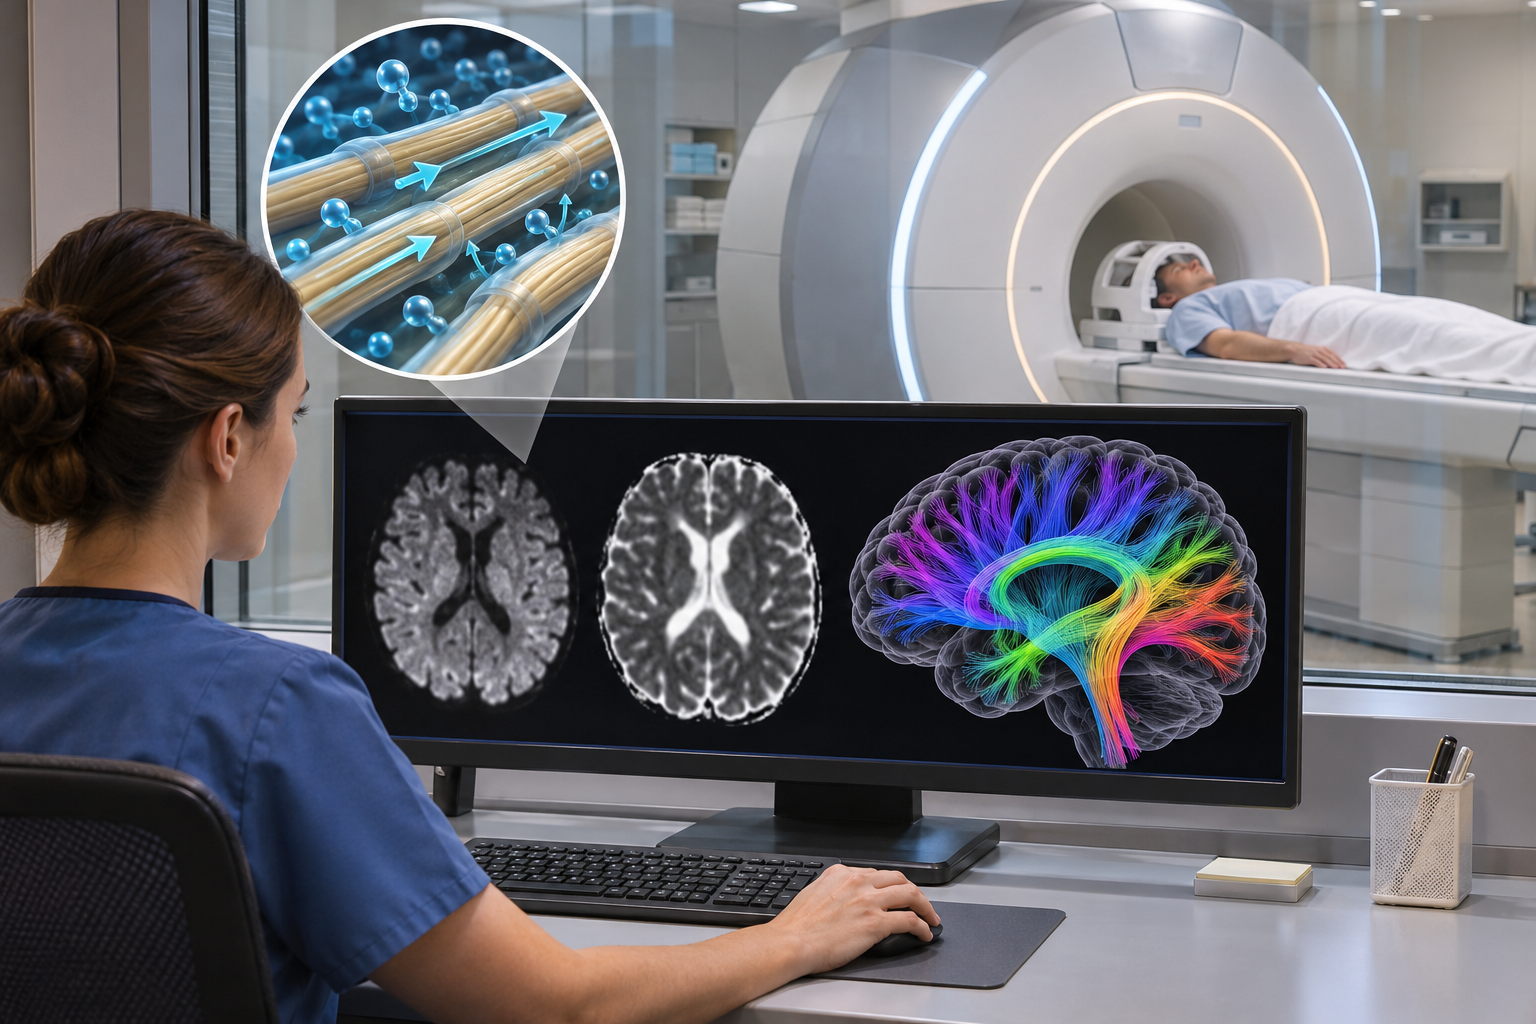
\includegraphics[width=\textwidth,keepaspectratio]{modalities/infographics/dmri_realistic.png}
\end{center}
\begin{center}\footnotesize Diffusion MRI is sensitive to microscopic water motion; DWI and ADC should be interpreted together, while tractography is model-derived. AI-generated illustration; displayed maps are not clinical studies.\end{center}

\section{Overview}
Diffusion magnetic resonance imaging (dMRI) is a specialized MRI technique that measures the microscopic movement of water molecules within biological tissues. This movement is influenced by cellular membranes, tissue microstructure, cellular density, viscosity, and the orientation of nerve fibers.

Unlike conventional MRI, which primarily provides anatomical information, diffusion MRI provides information about tissue microstructure and pathological changes that may not be visible on conventional MRI. It is particularly valuable for detecting acute cerebral ischemia, malignant tumors with high cellularity, abscesses and infections, white-matter injuries, demyelinating diseases, abnormalities of neural fiber pathways, and tumor response to treatment.

The 217 entries are a preliminary catalogue of diseases and conditions evaluated or investigated using diffusion MRI. They are not 217 independently validated clinical indications. Individual guideline and literature verification is necessary before using them as diagnostic ground truth.

\section{Where diffusion MRI is used}
The numbered entries give examples of reported diffusion MRI findings. Interpretation depends on acquisition technique, b-values, gradient directions, image quality, diffusion model, and correlation with ADC maps and other MRI sequences.

\subsection{Cerebrovascular diseases}
\begin{enumerate}[leftmargin=*,itemsep=0.45em,topsep=0.4em]
\item \textbf{Acute ischemic stroke.} Useful imaging findings include: Increased DWI signal and reduced ADC.
\item \textbf{Brainstem infarction.} Useful imaging findings include: Focal restricted diffusion within the brainstem.
\item \textbf{CADASIL.} Useful imaging findings include: Abnormal white-matter diffusion metrics.
\item \textbf{Cerebellar infarction.} Useful imaging findings include: Restricted diffusion within cerebellar tissue.
\item \textbf{Cerebral small vessel disease.} Useful imaging findings include: Reduced fractional anisotropy in affected white matter.
\item \textbf{Cerebral venous infarction.} Useful imaging findings include: Variable diffusion restriction and vasogenic edema.
\item \textbf{Delayed posthypoxic leukoencephalopathy.} Useful imaging findings include: Diffuse white-matter diffusion restriction.
\item \textbf{Global cerebral ischemia.} Useful imaging findings include: Widespread diffusion abnormalities.
\item \textbf{Hyperacute cerebral infarction.} Useful imaging findings include: Early diffusion restriction.
\item \textbf{Hypoxic-ischemic encephalopathy.} Useful imaging findings include: Cortical or deep gray-matter diffusion restriction.
\item \textbf{Lacunar infarction.} Useful imaging findings include: Small focal area of restricted diffusion.
\item \textbf{Moyamoya disease.} Useful imaging findings include: Ischemic lesions and altered white-matter integrity.
\item \textbf{Multiple embolic infarctions.} Useful imaging findings include: Multiple scattered areas of restricted diffusion.
\item \textbf{Posterior reversible encephalopathy syndrome.} Useful imaging findings include: Typically increased ADC due to vasogenic edema.
\item \textbf{Watershed infarction.} Useful imaging findings include: Restricted diffusion in arterial border zones.
\end{enumerate}
Acute ischemic stroke is among the most important and established clinical applications of diffusion MRI. DWI can be negative early, particularly with small or posterior-circulation infarcts; a negative scan does not exclude stroke when clinical suspicion remains. MRI should not delay time-critical treatment.

\subsection{Brain tumors}
\begin{enumerate}[leftmargin=*,itemsep=0.45em,topsep=0.4em]
\item \textbf{Atypical teratoid/rhabdoid tumor.} Useful imaging findings include: Restricted diffusion in solid components.
\item \textbf{Brain metastases.} Useful imaging findings include: Variable diffusion characteristics.
\item \textbf{Diffuse astrocytoma.} Useful imaging findings include: Variable ADC values.
\item \textbf{Embryonal tumor with multilayered rosettes.} Useful imaging findings include: Marked diffusion restriction.
\item \textbf{Ependymoma.} Useful imaging findings include: Variable diffusion restriction.
\item \textbf{Epidermoid cyst.} Useful imaging findings include: Characteristically increased DWI signal with reduced ADC relative to CSF.
\item \textbf{Germinoma.} Useful imaging findings include: Frequently reduced ADC.
\item \textbf{Glioblastoma.} Useful imaging findings include: Heterogeneous diffusion with restricted regions in cellular components.
\item \textbf{Hemangioblastoma.} Useful imaging findings include: Generally facilitated diffusion in solid components.
\item \textbf{Medulloblastoma.} Useful imaging findings include: Restricted diffusion associated with high cellularity.
\item \textbf{Meningioma.} Useful imaging findings include: Variable ADC, sometimes reduced in higher-grade tumors.
\item \textbf{Oligodendroglioma.} Useful imaging findings include: Variable intratumoral diffusion characteristics.
\item \textbf{Pilocytic astrocytoma.} Useful imaging findings include: Generally higher ADC in less cellular components.
\item \textbf{Pineoblastoma.} Useful imaging findings include: Restricted diffusion.
\item \textbf{Primary CNS lymphoma.} Useful imaging findings include: Markedly restricted diffusion.
\item \textbf{Radiation necrosis.} Useful imaging findings include: Variable diffusion characteristics, often overlapping with recurrence.
\item \textbf{Recurrent brain tumor.} Useful imaging findings include: Possible reduced ADC in viable tumor tissue.
\item \textbf{Vestibular schwannoma.} Useful imaging findings include: Variable diffusion characteristics.
\end{enumerate}
Diffusion measurements can support tumor characterization but cannot reliably establish histological or molecular tumor classification independently.

\subsection{Central nervous system infections}
\begin{enumerate}[leftmargin=*,itemsep=0.45em,topsep=0.4em]
\item \textbf{Cerebral malaria.} Useful imaging findings include: Variable cortical and white-matter diffusion abnormalities.
\item \textbf{Cerebral toxoplasmosis.} Useful imaging findings include: Variable diffusion characteristics.
\item \textbf{Epidural empyema.} Useful imaging findings include: Restricted diffusion within infectious collection.
\item \textbf{Fungal cerebral abscess.} Useful imaging findings include: Variable peripheral or central diffusion restriction.
\item \textbf{Herpes simplex encephalitis.} Useful imaging findings include: Restricted diffusion in temporal and insular regions.
\item \textbf{Intracranial tuberculoma.} Useful imaging findings include: Variable diffusion restriction depending on lesion composition.
\item \textbf{Japanese encephalitis.} Useful imaging findings include: Variable thalamic and deep gray-matter diffusion abnormalities.
\item \textbf{Progressive multifocal leukoencephalopathy.} Useful imaging findings include: Restricted diffusion at active lesion margins.
\item \textbf{Pyogenic cerebral abscess.} Useful imaging findings include: Marked central diffusion restriction.
\item \textbf{Subdural empyema.} Useful imaging findings include: Restricted diffusion within purulent collection.
\item \textbf{Tuberculous abscess.} Useful imaging findings include: Restricted diffusion within purulent material.
\item \textbf{Ventriculitis.} Useful imaging findings include: Restricted diffusion within ventricular debris.
\item \textbf{West Nile encephalitis.} Useful imaging findings include: Possible diffusion restriction in affected neural structures.
\end{enumerate}

\subsection{Demyelinating and white-matter diseases}
\begin{enumerate}[leftmargin=*,itemsep=0.45em,topsep=0.4em]
\item \textbf{Acute disseminated encephalomyelitis.} Useful imaging findings include: Variable diffusion abnormalities.
\item \textbf{Alexander disease.} Useful imaging findings include: Altered white-matter diffusion characteristics.
\item \textbf{Canavan disease.} Useful imaging findings include: Abnormal white-matter diffusion.
\item \textbf{Krabbe disease.} Useful imaging findings include: Altered diffusion in affected white-matter tracts.
\item \textbf{Metachromatic leukodystrophy.} Useful imaging findings include: Abnormal white-matter diffusion metrics.
\item \textbf{MOG antibody-associated disease.} Useful imaging findings include: Variable lesional diffusion abnormalities.
\item \textbf{Multiple sclerosis.} Useful imaging findings include: Altered ADC and reduced fractional anisotropy.
\item \textbf{Neuromyelitis optica spectrum disorder.} Useful imaging findings include: Altered diffusion within affected neural pathways.
\item \textbf{Osmotic demyelination syndrome.} Useful imaging findings include: Early diffusion restriction in affected regions.
\item \textbf{Toxic leukoencephalopathy.} Useful imaging findings include: Symmetric white-matter diffusion restriction.
\item \textbf{Vanishing white matter disease.} Useful imaging findings include: Increased diffusivity in degenerating white matter.
\item \textbf{X-linked adrenoleukodystrophy.} Useful imaging findings include: Abnormal diffusion within demyelinating regions.
\end{enumerate}

\subsection{Neurodegenerative diseases}
\begin{enumerate}[leftmargin=*,itemsep=0.45em,topsep=0.4em]
\item \textbf{Alzheimer disease.} Useful imaging findings include: Reduced white-matter integrity and altered diffusivity.
\item \textbf{Amyotrophic lateral sclerosis.} Useful imaging findings include: Reduced fractional anisotropy in corticospinal tracts.
\item \textbf{Creutzfeldt--Jakob disease.} Useful imaging findings include: Cortical ribboning and basal ganglia diffusion restriction.
\item \textbf{Dementia with Lewy bodies.} Useful imaging findings include: Altered white-matter microstructure.
\item \textbf{Friedreich ataxia.} Useful imaging findings include: Altered diffusion in cerebellar and spinal pathways.
\item \textbf{Frontotemporal dementia.} Useful imaging findings include: Abnormal frontal and temporal white-matter diffusion.
\item \textbf{Huntington disease.} Useful imaging findings include: Altered corticostriatal diffusion metrics.
\item \textbf{Mild cognitive impairment.} Useful imaging findings include: Altered hippocampal and white-matter diffusion metrics.
\item \textbf{Multiple system atrophy.} Useful imaging findings include: Increased diffusivity in affected subcortical structures.
\item \textbf{Parkinson disease.} Useful imaging findings include: Altered diffusion in nigrostriatal pathways.
\item \textbf{Primary lateral sclerosis.} Useful imaging findings include: Altered corticospinal tract integrity.
\item \textbf{Progressive supranuclear palsy.} Useful imaging findings include: Abnormal brainstem diffusion metrics.
\item \textbf{Spinocerebellar ataxia.} Useful imaging findings include: Altered cerebellar white-matter integrity.
\item \textbf{Wilson disease.} Useful imaging findings include: Abnormal diffusion within basal ganglia.
\end{enumerate}
Except for selected conditions such as Creutzfeldt--Jakob disease, most diffusion biomarkers in neurodegenerative diseases remain supplementary or investigational.

\subsection{Traumatic brain injuries}
\begin{enumerate}[leftmargin=*,itemsep=0.45em,topsep=0.4em]
\item \textbf{Cerebral contusion.} Useful imaging findings include: Variable diffusion restriction and edema.
\item \textbf{Diffuse axonal injury.} Useful imaging findings include: Abnormal diffusion within injured white-matter tracts.
\item \textbf{Mild traumatic brain injury.} Useful imaging findings include: Variable white-matter diffusion metrics.
\item \textbf{Moderate traumatic brain injury.} Useful imaging findings include: Altered white-matter microstructure.
\item \textbf{Post-concussion syndrome.} Useful imaging findings include: Reported alterations in white-matter integrity.
\item \textbf{Severe traumatic brain injury.} Useful imaging findings include: Widespread diffusion abnormalities.
\item \textbf{Traumatic brainstem injury.} Useful imaging findings include: Abnormal diffusion within brainstem pathways.
\item \textbf{Traumatic corpus callosum injury.} Useful imaging findings include: Altered callosal diffusion characteristics.
\end{enumerate}

\subsection{Neurodevelopmental and psychiatric disorders}
\begin{enumerate}[leftmargin=*,itemsep=0.45em,topsep=0.4em]
\item \textbf{Attention deficit hyperactivity disorder.} Useful imaging findings include: Altered diffusion in executive control pathways.
\item \textbf{Autism spectrum disorder.} Useful imaging findings include: Reported alterations in white-matter connectivity.
\item \textbf{Bipolar disorder.} Useful imaging findings include: Altered frontolimbic white-matter integrity.
\item \textbf{Cerebral palsy.} Useful imaging findings include: Abnormal corticospinal tract development.
\item \textbf{Developmental dyslexia.} Useful imaging findings include: Altered language-related white-matter tracts.
\item \textbf{Down syndrome.} Useful imaging findings include: Altered white-matter development.
\item \textbf{Fragile X syndrome.} Useful imaging findings include: Abnormal white-matter microstructure.
\item \textbf{Major depressive disorder.} Useful imaging findings include: Reported abnormalities in frontolimbic connectivity.
\item \textbf{Obsessive-compulsive disorder.} Useful imaging findings include: Altered corticostriatal white-matter pathways.
\item \textbf{Post-traumatic stress disorder.} Useful imaging findings include: Altered limbic white-matter connectivity.
\item \textbf{Schizophrenia.} Useful imaging findings include: Reduced fractional anisotropy in selected white-matter pathways.
\item \textbf{Tourette syndrome.} Useful imaging findings include: Altered corticostriatal diffusion metrics.
\end{enumerate}
These applications are predominantly research-oriented. Diffusion MRI cannot independently diagnose these psychiatric or neurodevelopmental disorders.

\subsection{Spinal cord and peripheral nerves}
\begin{enumerate}[leftmargin=*,itemsep=0.45em,topsep=0.4em]
\item \textbf{Brachial plexus injury.} Useful imaging findings include: Altered diffusion and fiber tract continuity.
\item \textbf{Carpal tunnel syndrome.} Useful imaging findings include: Altered median nerve diffusion metrics.
\item \textbf{Cervical spondylotic myelopathy.} Useful imaging findings include: Reduced fractional anisotropy.
\item \textbf{Compressive myelopathy.} Useful imaging findings include: Altered spinal cord diffusion metrics.
\item \textbf{Diabetic peripheral neuropathy.} Useful imaging findings include: Reported changes in peripheral nerve diffusion metrics.
\item \textbf{Multiple sclerosis of the spinal cord.} Useful imaging findings include: Abnormal diffusion in demyelinating lesions.
\item \textbf{Spinal cord infarction.} Useful imaging findings include: Restricted intramedullary diffusion.
\item \textbf{Spinal cord tumors.} Useful imaging findings include: Variable ADC and displacement of neural tracts.
\item \textbf{Transverse myelitis.} Useful imaging findings include: Variable intramedullary diffusion abnormalities.
\item \textbf{Traumatic spinal cord injury.} Useful imaging findings include: Altered diffusion within injured spinal pathways.
\item \textbf{Ulnar nerve entrapment.} Useful imaging findings include: Abnormal diffusion within the affected nerve.
\end{enumerate}

\subsection{Head and neck diseases}
\begin{enumerate}[leftmargin=*,itemsep=0.45em,topsep=0.4em]
\item \textbf{Cholesteatoma.} Useful imaging findings include: Marked DWI hyperintensity on dedicated sequences.
\item \textbf{Deep neck abscess.} Useful imaging findings include: Central diffusion restriction.
\item \textbf{Head and neck lymphoma.} Useful imaging findings include: Marked diffusion restriction.
\item \textbf{Laryngeal carcinoma.} Useful imaging findings include: Reduced tumor ADC.
\item \textbf{Malignant salivary gland tumor.} Useful imaging findings include: Variable or reduced ADC.
\item \textbf{Metastatic cervical lymphadenopathy.} Useful imaging findings include: Variable diffusion restriction.
\item \textbf{Nasopharyngeal carcinoma.} Useful imaging findings include: Reduced ADC in cellular tumor regions.
\item \textbf{Oral squamous cell carcinoma.} Useful imaging findings include: Restricted diffusion in viable tumor.
\item \textbf{Orbital lymphoma.} Useful imaging findings include: Marked diffusion restriction.
\item \textbf{Pleomorphic adenoma.} Useful imaging findings include: Generally higher ADC than highly cellular tumors.
\item \textbf{Retinoblastoma.} Useful imaging findings include: Restricted diffusion within solid tumor.
\item \textbf{Warthin tumor.} Useful imaging findings include: Frequently low ADC.
\end{enumerate}

\subsection{Breast diseases}
\begin{enumerate}[leftmargin=*,itemsep=0.45em,topsep=0.4em]
\item \textbf{Breast abscess.} Useful imaging findings include: Restricted diffusion within purulent material.
\item \textbf{Breast cancer response to chemotherapy.} Useful imaging findings include: Often increased ADC following effective treatment.
\item \textbf{Breast lymphoma.} Useful imaging findings include: Marked diffusion restriction.
\item \textbf{Ductal carcinoma in situ.} Useful imaging findings include: Variable ADC depending on cellularity.
\item \textbf{Fibroadenoma.} Useful imaging findings include: Frequently higher ADC than malignant lesions.
\item \textbf{Invasive ductal carcinoma.} Useful imaging findings include: Frequently reduced ADC.
\item \textbf{Invasive lobular carcinoma.} Useful imaging findings include: Variable diffusion restriction.
\item \textbf{Phyllodes tumor.} Useful imaging findings include: Variable diffusion characteristics.
\item \textbf{Residual breast cancer.} Useful imaging findings include: Persistent diffusion restriction in some viable tumor regions.
\item \textbf{Triple-negative breast cancer.} Useful imaging findings include: Heterogeneous diffusion characteristics.
\end{enumerate}

\subsection{Liver and biliary diseases}
\begin{enumerate}[leftmargin=*,itemsep=0.45em,topsep=0.4em]
\item \textbf{Extrahepatic cholangiocarcinoma.} Useful imaging findings include: Restricted diffusion in affected tissue.
\item \textbf{Focal nodular hyperplasia.} Useful imaging findings include: Variable diffusion characteristics.
\item \textbf{Gallbladder carcinoma.} Useful imaging findings include: Restricted diffusion within malignant tissue.
\item \textbf{Hepatic adenoma.} Useful imaging findings include: Variable ADC.
\item \textbf{Hepatic hemangioma.} Useful imaging findings include: Generally high ADC despite possible DWI hyperintensity.
\item \textbf{Hepatic metastases.} Useful imaging findings include: Restricted diffusion, particularly in viable cellular regions.
\item \textbf{Hepatocellular carcinoma.} Useful imaging findings include: Frequently restricted diffusion in viable tumor.
\item \textbf{Intrahepatic cholangiocarcinoma.} Useful imaging findings include: Restricted diffusion in solid tumor components.
\item \textbf{Liver abscess.} Useful imaging findings include: Central diffusion restriction.
\item \textbf{Liver cirrhosis.} Useful imaging findings include: Altered parenchymal diffusion metrics.
\item \textbf{Liver fibrosis.} Useful imaging findings include: Possible reduction in ADC.
\item \textbf{Simple hepatic cyst.} Useful imaging findings include: Facilitated diffusion.
\end{enumerate}

\subsection{Pancreatic diseases}
\begin{enumerate}[leftmargin=*,itemsep=0.45em,topsep=0.4em]
\item \textbf{Acute pancreatitis.} Useful imaging findings include: Altered pancreatic diffusion.
\item \textbf{Autoimmune pancreatitis.} Useful imaging findings include: Diffuse or focal diffusion restriction.
\item \textbf{Chronic pancreatitis.} Useful imaging findings include: Variable reduction in ADC.
\item \textbf{Intraductal papillary mucinous neoplasm.} Useful imaging findings include: Variable restriction in suspicious solid components.
\item \textbf{Pancreatic abscess.} Useful imaging findings include: Restricted diffusion within purulent material.
\item \textbf{Pancreatic ductal adenocarcinoma.} Useful imaging findings include: Frequently reduced ADC.
\item \textbf{Pancreatic neuroendocrine tumor.} Useful imaging findings include: Variable diffusion restriction.
\item \textbf{Solid pseudopapillary neoplasm.} Useful imaging findings include: Variable diffusion in solid components.
\end{enumerate}

\subsection{Gastrointestinal diseases}
\begin{enumerate}[leftmargin=*,itemsep=0.45em,topsep=0.4em]
\item \textbf{Active Crohn disease.} Useful imaging findings include: Restricted diffusion within inflamed bowel wall.
\item \textbf{Acute appendicitis.} Useful imaging findings include: Possible diffusion restriction in inflamed appendix.
\item \textbf{Anal carcinoma.} Useful imaging findings include: Restricted diffusion in tumor tissue.
\item \textbf{Colorectal carcinoma.} Useful imaging findings include: Reduced tumor ADC.
\item \textbf{Esophageal carcinoma.} Useful imaging findings include: Restricted diffusion in viable tumor.
\item \textbf{Gastric carcinoma.} Useful imaging findings include: Variable tumor diffusion restriction.
\item \textbf{Gastrointestinal lymphoma.} Useful imaging findings include: Marked diffusion restriction.
\item \textbf{Gastrointestinal stromal tumor.} Useful imaging findings include: Variable diffusion characteristics.
\item \textbf{Perianal abscess.} Useful imaging findings include: Restricted diffusion within purulent collection.
\item \textbf{Peritoneal carcinomatosis.} Useful imaging findings include: Diffusion restriction within metastatic deposits.
\item \textbf{Rectal carcinoma.} Useful imaging findings include: Restricted diffusion within viable tumor.
\item \textbf{Residual rectal carcinoma after treatment.} Useful imaging findings include: Persistent focal diffusion restriction in some cases.
\item \textbf{Ulcerative colitis.} Useful imaging findings include: Altered diffusion in inflamed colonic tissue.
\end{enumerate}

\subsection{Renal and urinary diseases}
\begin{enumerate}[leftmargin=*,itemsep=0.45em,topsep=0.4em]
\item \textbf{Acute pyelonephritis.} Useful imaging findings include: Focal or regional diffusion restriction.
\item \textbf{Bladder carcinoma.} Useful imaging findings include: Restricted diffusion within viable tumor.
\item \textbf{Chromophobe renal cell carcinoma.} Useful imaging findings include: Variable or reduced ADC.
\item \textbf{Chronic kidney disease.} Useful imaging findings include: Altered cortical and medullary diffusivity.
\item \textbf{Clear cell renal cell carcinoma.} Useful imaging findings include: Variable ADC.
\item \textbf{Papillary renal cell carcinoma.} Useful imaging findings include: Frequently lower ADC than clear cell carcinoma.
\item \textbf{Renal abscess.} Useful imaging findings include: Marked central diffusion restriction.
\item \textbf{Renal fibrosis.} Useful imaging findings include: Altered renal diffusion parameters.
\item \textbf{Renal infarction.} Useful imaging findings include: Regional diffusion restriction.
\item \textbf{Renal lymphoma.} Useful imaging findings include: Marked diffusion restriction.
\item \textbf{Renal oncocytoma.} Useful imaging findings include: Variable diffusion characteristics.
\item \textbf{Urothelial carcinoma.} Useful imaging findings include: Restricted diffusion within tumor.
\end{enumerate}

\subsection{Female reproductive system}
\begin{enumerate}[leftmargin=*,itemsep=0.45em,topsep=0.4em]
\item \textbf{Adenomyosis.} Useful imaging findings include: Variable myometrial diffusion abnormalities.
\item \textbf{Cellular uterine leiomyoma.} Useful imaging findings include: May show marked diffusion restriction and low ADC, overlapping with leiomyosarcoma.
\item \textbf{Cervical carcinoma.} Useful imaging findings include: Reduced tumor ADC.
\item \textbf{Degenerating uterine fibroid.} Useful imaging findings include: Variable diffusion characteristics.
\item \textbf{Dysgerminoma.} Useful imaging findings include: Restricted diffusion in solid tumor.
\item \textbf{Endometrial carcinoma.} Useful imaging findings include: Restricted diffusion within malignant tissue.
\item \textbf{Endometrioma.} Useful imaging findings include: Variable restriction related to hemorrhagic contents.
\item \textbf{Granulosa cell tumor.} Useful imaging findings include: Variable diffusion characteristics.
\item \textbf{Ovarian carcinoma.} Useful imaging findings include: Restricted diffusion in solid tumor components.
\item \textbf{Ovarian torsion.} Useful imaging findings include: Possible diffusion restriction due to ischemia.
\item \textbf{Pelvic lymph node metastases.} Useful imaging findings include: Variable diffusion restriction.
\item \textbf{Tubo-ovarian abscess.} Useful imaging findings include: Restricted diffusion in purulent components.
\item \textbf{Uterine leiomyosarcoma.} Useful imaging findings include: Frequently reduced ADC in viable cellular components.
\end{enumerate}

\subsection{Male reproductive system}
\begin{enumerate}[leftmargin=*,itemsep=0.45em,topsep=0.4em]
\item \textbf{Benign prostatic hyperplasia.} Useful imaging findings include: Variable ADC in hyperplastic nodules.
\item \textbf{Nonseminomatous germ cell tumor.} Useful imaging findings include: Heterogeneous diffusion characteristics.
\item \textbf{Penile carcinoma.} Useful imaging findings include: Restricted diffusion within malignant tissue.
\item \textbf{Prostate adenocarcinoma.} Useful imaging findings include: High DWI signal and reduced ADC.
\item \textbf{Prostatic abscess.} Useful imaging findings include: Marked central diffusion restriction.
\item \textbf{Prostatitis.} Useful imaging findings include: Possible diffusion restriction mimicking malignancy.
\item \textbf{Testicular infarction.} Useful imaging findings include: Focal diffusion restriction.
\item \textbf{Testicular seminoma.} Useful imaging findings include: Frequently reduced ADC.
\item \textbf{Testicular torsion.} Useful imaging findings include: Possible restricted diffusion associated with ischemia; MRI is not the routine initial test for acute scrotal pain.
\end{enumerate}
Diffusion-weighted imaging is a key component of standardized prostate MRI assessment, but it is interpreted with anatomical sequences and the clinical context rather than used as a stand-alone test.

For suspected acute testicular torsion, ultrasound is generally the initial imaging examination when imaging is needed. MRI should not delay urgent clinical or surgical assessment.

\subsection{Musculoskeletal diseases}
\begin{enumerate}[leftmargin=*,itemsep=0.45em,topsep=0.4em]
\item \textbf{Bone lymphoma.} Useful imaging findings include: Marked diffusion restriction.
\item \textbf{Bone metastases.} Useful imaging findings include: Altered diffusion in marrow-replacing lesions.
\item \textbf{Chondrosarcoma.} Useful imaging findings include: Variable ADC influenced by cartilaginous matrix.
\item \textbf{Ewing sarcoma.} Useful imaging findings include: Frequently reduced ADC.
\item \textbf{Intraosseous abscess.} Useful imaging findings include: Restricted diffusion within purulent material.
\item \textbf{Malignant peripheral nerve sheath tumor.} Useful imaging findings include: Frequently reduced ADC in cellular regions.
\item \textbf{Multiple myeloma.} Useful imaging findings include: Abnormal marrow diffusion characteristics.
\item \textbf{Muscle ischemia.} Useful imaging findings include: Abnormal diffusion within affected muscle.
\item \textbf{Muscular dystrophy.} Useful imaging findings include: Altered muscle fiber diffusion metrics.
\item \textbf{Myositis.} Useful imaging findings include: Altered muscle diffusion characteristics.
\item \textbf{Osteomyelitis.} Useful imaging findings include: Variable diffusion restriction in infected marrow.
\item \textbf{Osteosarcoma.} Useful imaging findings include: Restricted diffusion in viable cellular tumor.
\item \textbf{Peripheral nerve sheath tumor.} Useful imaging findings include: Variable ADC.
\item \textbf{Rhabdomyosarcoma.} Useful imaging findings include: Restricted diffusion in cellular tumor.
\item \textbf{Septic arthritis.} Useful imaging findings include: Variable restriction within infectious collections.
\item \textbf{Soft-tissue abscess.} Useful imaging findings include: Central diffusion restriction.
\item \textbf{Soft-tissue sarcoma.} Useful imaging findings include: Variable ADC associated with tumor composition.
\end{enumerate}

\subsection{Fetal and neonatal disorders}
\begin{enumerate}[leftmargin=*,itemsep=0.45em,topsep=0.4em]
\item \textbf{Congenital white-matter abnormalities.} Useful imaging findings include: Altered developmental diffusion metrics.
\item \textbf{Fetal cerebral ischemia.} Useful imaging findings include: Restricted diffusion in affected tissue.
\item \textbf{Neonatal cerebral infarction.} Useful imaging findings include: Focal restricted diffusion.
\item \textbf{Neonatal encephalitis.} Useful imaging findings include: Variable diffusion restriction.
\item \textbf{Neonatal hypoglycemic brain injury.} Useful imaging findings include: Predominantly posterior diffusion abnormalities in many cases.
\item \textbf{Neonatal hypoxic-ischemic encephalopathy.} Useful imaging findings include: Characteristic regional diffusion restriction.
\item \textbf{Periventricular leukomalacia.} Useful imaging findings include: Abnormal periventricular white-matter diffusion.
\item \textbf{Prematurity-associated brain injury.} Useful imaging findings include: Altered white-matter development and diffusion.
\end{enumerate}

\subsection{Summary of catalogue}
\begin{center}
\begin{tabular}{@{}p{0.70\textwidth}r@{}}
\toprule
\textbf{Disease category} & \textbf{Entries} \\
\midrule
Brain tumors & 18 \\
Breast diseases & 10 \\
Central nervous system infections & 13 \\
Cerebrovascular diseases & 15 \\
Demyelinating and white-matter diseases & 12 \\
Female reproductive system & 13 \\
Fetal and neonatal disorders & 8 \\
Gastrointestinal diseases & 13 \\
Head and neck diseases & 12 \\
Liver and biliary diseases & 12 \\
Male reproductive system & 9 \\
Musculoskeletal diseases & 17 \\
Neurodegenerative diseases & 14 \\
Neurodevelopmental and psychiatric disorders & 12 \\
Pancreatic diseases & 8 \\
Renal and urinary diseases & 12 \\
Spinal cord and peripheral nerves & 11 \\
Total & 217 \\
Traumatic brain injuries & 8 \\
\bottomrule
\end{tabular}
\end{center}

\subsection{Types of diffusion MRI}
Diffusion MRI is an umbrella term for distinct acquisition and mathematical modeling techniques.
\begin{longtable}{@{}p{0.30\textwidth}p{0.14\textwidth}p{0.48\textwidth}@{}}
\toprule
\textbf{Technique} & \textbf{Abbreviation} & \textbf{Primary application} \\
\midrule
\endfirsthead
\toprule
\textbf{Technique} & \textbf{Abbreviation} & \textbf{Primary application} \\
\midrule
\endhead
Apparent diffusion coefficient mapping & ADC & Quantitative estimation of diffusivity \\
Diffusion kurtosis imaging & DKI & Non-Gaussian diffusion characterization \\
Diffusion spectrum imaging & DSI & Complex fiber orientation estimation \\
Diffusion tensor imaging & DTI & Directional diffusion and tissue anisotropy \\
Diffusion tensor tractography & DTT & Visualization of estimated neural fiber pathways \\
Diffusion-weighted imaging & DWI & Detection of diffusion abnormalities \\
Diffusion-weighted spectroscopy & DWS & Diffusion characteristics of tissue metabolites \\
Free-water diffusion imaging & FW-DTI & Estimation of extracellular free-water contribution \\
High angular resolution diffusion imaging & HARDI & Estimation of crossing fiber orientations \\
Intravoxel incoherent motion imaging & IVIM & Separation of diffusion and microvascular contributions \\
Microscopic fractional anisotropy & $\mu$FA & Estimation of microscopic diffusion anisotropy \\
Neurite orientation dispersion and density imaging & NODDI & Modeling neurite microstructure \\
Restriction spectrum imaging & RSI & Separation of diffusion components \\
Spherical mean technique & SMT & Tissue microstructure characterization \\
\bottomrule
\end{longtable}

\subsection{Quantitative diffusion parameters}
\begin{longtable}{@{}p{0.34\textwidth}p{0.16\textwidth}p{0.42\textwidth}@{}}
\toprule
\textbf{Parameter} & \textbf{Abbreviation} & \textbf{Interpretation} \\
\midrule
\endfirsthead
\toprule
\textbf{Parameter} & \textbf{Abbreviation} & \textbf{Interpretation} \\
\midrule
\endhead
Apparent diffusion coefficient & ADC & Apparent magnitude of water diffusion \\
Axial diffusivity & AD & Diffusion along the principal tensor direction \\
Axial kurtosis & AK & Non-Gaussian diffusion along the principal direction \\
Diffusion weighting factor & $b$-value & Strength of diffusion sensitization \\
Fractional anisotropy & FA & Degree of directional diffusion anisotropy \\
Free-water fraction & FWF & Estimated extracellular free-water contribution \\
Mean diffusivity & MD & Average diffusion magnitude \\
Mean kurtosis & MK & Average deviation from Gaussian diffusion \\
Neurite density index & NDI & Model-derived neurite density estimate \\
Orientation dispersion index & ODI & Model-derived variation in neurite orientation \\
Perfusion fraction & $f$ & Estimated microvascular signal contribution in IVIM \\
Pseudodiffusion coefficient & $D^*$ & Estimated microvascular-related diffusivity \\
Radial diffusivity & RD & Average diffusion perpendicular to the principal direction \\
Radial kurtosis & RK & Non-Gaussian diffusion perpendicular to the principal direction \\
True diffusion coefficient & $D$ & Estimated tissue diffusion component in IVIM \\
\bottomrule
\end{longtable}

Diffusion metrics are indirect and model-dependent. Fractional anisotropy and related measures are not specific markers of axonal integrity, myelin, or a particular disease. Tractography estimates possible pathways from water-diffusion data; it does not directly image or trace axons, and crossing fibers can lead to missed or spurious pathways.

\subsection{Physical interpretation of diffusion-weighted imaging}
Under a simplified monoexponential diffusion model,
\begin{equation}
S(b)=S_0 e^{-b\,ADC},
\end{equation}
where $S(b)$ is the diffusion-weighted signal intensity, $S_0$ is the signal without diffusion weighting, $b$ is the diffusion weighting factor measured in s/mm$^2$, and ADC is the apparent diffusion coefficient measured in mm$^2$/s.

For diffusion tensor imaging, the diffusion tensor is represented by a symmetric matrix:
\begin{equation}
\mathbf{D}=\begin{bmatrix}
D_{xx}&D_{xy}&D_{xz}\\
D_{xy}&D_{yy}&D_{yz}\\
D_{xz}&D_{yz}&D_{zz}
\end{bmatrix}.
\end{equation}
Its eigenvalues $\lambda_1,\lambda_2,\lambda_3$ are used to calculate mean diffusivity and fractional anisotropy:
\begin{equation}
MD=\frac{\lambda_1+\lambda_2+\lambda_3}{3}
\end{equation}
\begin{equation}
FA=\sqrt{\frac{3}{2}}\sqrt{\frac{(\lambda_1-MD)^2+(\lambda_2-MD)^2+(\lambda_3-MD)^2}{\lambda_1^2+\lambda_2^2+\lambda_3^2}}.
\end{equation}

\subsection{Established clinical applications versus research applications}
\begin{longtable}{@{}p{0.45\textwidth}p{0.49\textwidth}@{}}
\toprule
\textbf{Application} & \textbf{Clinical status} \\
\midrule
Acute ischemic stroke detection & Established \\
Brain tumor characterization & Established supplementary technique \\
Breast cancer characterization & Established supplementary technique \\
Cerebral abscess characterization & Established \\
Cholesteatoma detection & Established \\
Creutzfeldt--Jakob disease assessment & Established \\
Liver metastasis detection & Established supplementary technique \\
Mild traumatic brain injury diagnosis using DTI & Investigational \\
Neonatal hypoxic-ischemic injury & Established \\
Neurodegenerative disease classification & Predominantly research \\
Neurodevelopmental disease diagnosis & Experimental \\
Peripheral nerve microstructure assessment & Emerging \\
Presurgical neural tract mapping & Specialized clinical application \\
Prostate cancer detection & Established \\
Psychiatric disease diagnosis & Experimental \\
Rectal cancer treatment response assessment & Established \\
Whole-body multiple myeloma assessment & Established \\
\bottomrule
\end{longtable}

\subsection{Selected clinical guidance and methodological references}
The following sources support the clinical and interpretation limitations described above:
\begin{itemize}
\item \href{https://pmc.ncbi.nlm.nih.gov/articles/PMC5513816/}{Meta-analysis of DWI-negative acute ischemic stroke} (early and posterior-circulation infarcts may be missed).
\item \href{https://acsearch.acr.org/docs/69363/Narrative}{ACR Appropriateness Criteria: Acute Onset of Scrotal Pain} (ultrasound is generally the initial examination).
\item \href{https://pubs.rsna.org/radiographics/doi/full/10.1148/radiol.211658}{RSNA consensus statement on MRI evaluation of uterine masses} (restricted diffusion can overlap between cellular leiomyoma and leiomyosarcoma).
\item \href{https://www.acr.org/-/media/ACR/Files/RADS/PI-RADS/PIRADS-V2-1.pdf}{ACR PI-RADS v2.1} (DWI is interpreted within a standardized prostate MRI assessment).
\item \href{https://pmc.ncbi.nlm.nih.gov/articles/PMC3119814/}{Review of diffusion tractography} (streamlines are estimates and have known limitations in crossing or complex fiber regions).
\end{itemize}

\subsection{Published diffusion MRI datasets}
\begin{longtable}{@{}p{0.36\textwidth}p{0.58\textwidth}@{}}
\toprule
\textbf{Source} & \textbf{Primary utility} \\
\midrule
\endfirsthead
\toprule
\textbf{Source} & \textbf{Primary utility} \\
\midrule
\endhead
ADNI & Neurodegenerative diseases \\
Developing Human Connectome Project & Neonatal brain development \\
DIPY & Diffusion MRI computational algorithms \\
Human Connectome Project & High-resolution brain diffusion MRI \\
ISLES Challenge & Ischemic stroke imaging and segmentation \\
MRtrix3 & Diffusion modeling and tractography \\
OpenNeuro & Public neuroimaging datasets \\
PubMed Central & Published clinical diffusion MRI images \\
The Cancer Imaging Archive & Oncological diffusion MRI \\
UK Biobank & Population-scale diffusion imaging \\
\bottomrule
\end{longtable}

\subsection{Recommended metadata for a diffusion MRI dataset}
\begin{longtable}{@{}p{0.45\textwidth}p{0.49\textwidth}@{}}
\toprule
\textbf{Attribute} & \textbf{Example} \\
\midrule
$b$-values & 0, 1000, 2000 s/mm$^2$ \\
Acquisition technique & DWI \\
ADC & $0.55 \times 10^{-3}$ mm$^2$/s \\
Anatomical region & Brain \\
Dataset organization & BIDS \\
Derived maps & ADC, FA, MD \\
Diagnostic reference standard & Independently confirmed clinical diagnosis \\
Diffusion model & Tensor \\
Disease & Acute ischemic stroke \\
Eddy-current correction & Applied \\
Fractional anisotropy & 0.42 \\
Gradient information & bval and bvec files \\
Image format & DICOM or NIfTI \\
Image orientation & Axial \\
Imaging modality & Diffusion MRI \\
Magnetic field strength & 3 Tesla \\
Motion correction & Applied \\
Number of diffusion directions & 64 \\
Publication reference & DOI or PMID \\
Susceptibility distortion correction & Applied \\
Voxel dimensions & $2 \times 2 \times 2$ mm \\
\bottomrule
\end{longtable}

\subsection{Data dimensionality and interpretation}
Unlike fMRI, in which the fourth dimension generally represents time, in diffusion MRI the fourth dimension generally represents different diffusion weightings and gradient directions.
\begin{center}
\begin{tabular}{@{}ll@{}}
\toprule
\textbf{Modality} & \textbf{Data dimensionality} \\
\midrule
CT & $X, Y, Z$ \\
Diffusion MRI & $X, Y, Z$, diffusion encoding \\
Diffusion tensor imaging & $X, Y, Z$, tensor components \\
Diffusion tractography & Three-dimensional estimated fiber trajectories \\
Functional MRI & $X, Y, Z$, time \\
Structural MRI & $X, Y, Z$ per sequence \\
\bottomrule
\end{tabular}
\end{center}

A key interpretation issue is distinguishing true diffusion restriction from T2 shine-through:
\begin{center}
\begin{tabular}{@{}lll@{}}
\toprule
\textbf{Finding} & \textbf{DWI signal} & \textbf{ADC signal} \\
\midrule
Facilitated diffusion & Often low & High \\
T2 shine-through & High & Normal or high \\
True diffusion restriction & High & Low \\
\bottomrule
\end{tabular}
\end{center}
Consequently, a diffusion-weighted image should generally be interpreted alongside its corresponding ADC map and relevant anatomical MRI sequences.

The 217 entries constitute a preliminary catalogue of diseases and conditions evaluated or investigated using diffusion MRI. They are not independently validated clinical indications; individual guideline and literature verification is necessary before using them as diagnostic ground truth.
